\documentclass[border=6pt]{standalone}
\usepackage{tikz}
\usetikzlibrary{arrows.meta,positioning,fit,backgrounds,calc}
\usepackage[T1]{fontenc}
\usepackage{lmodern}
\usepackage[none]{hyphenat}
\begin{document}
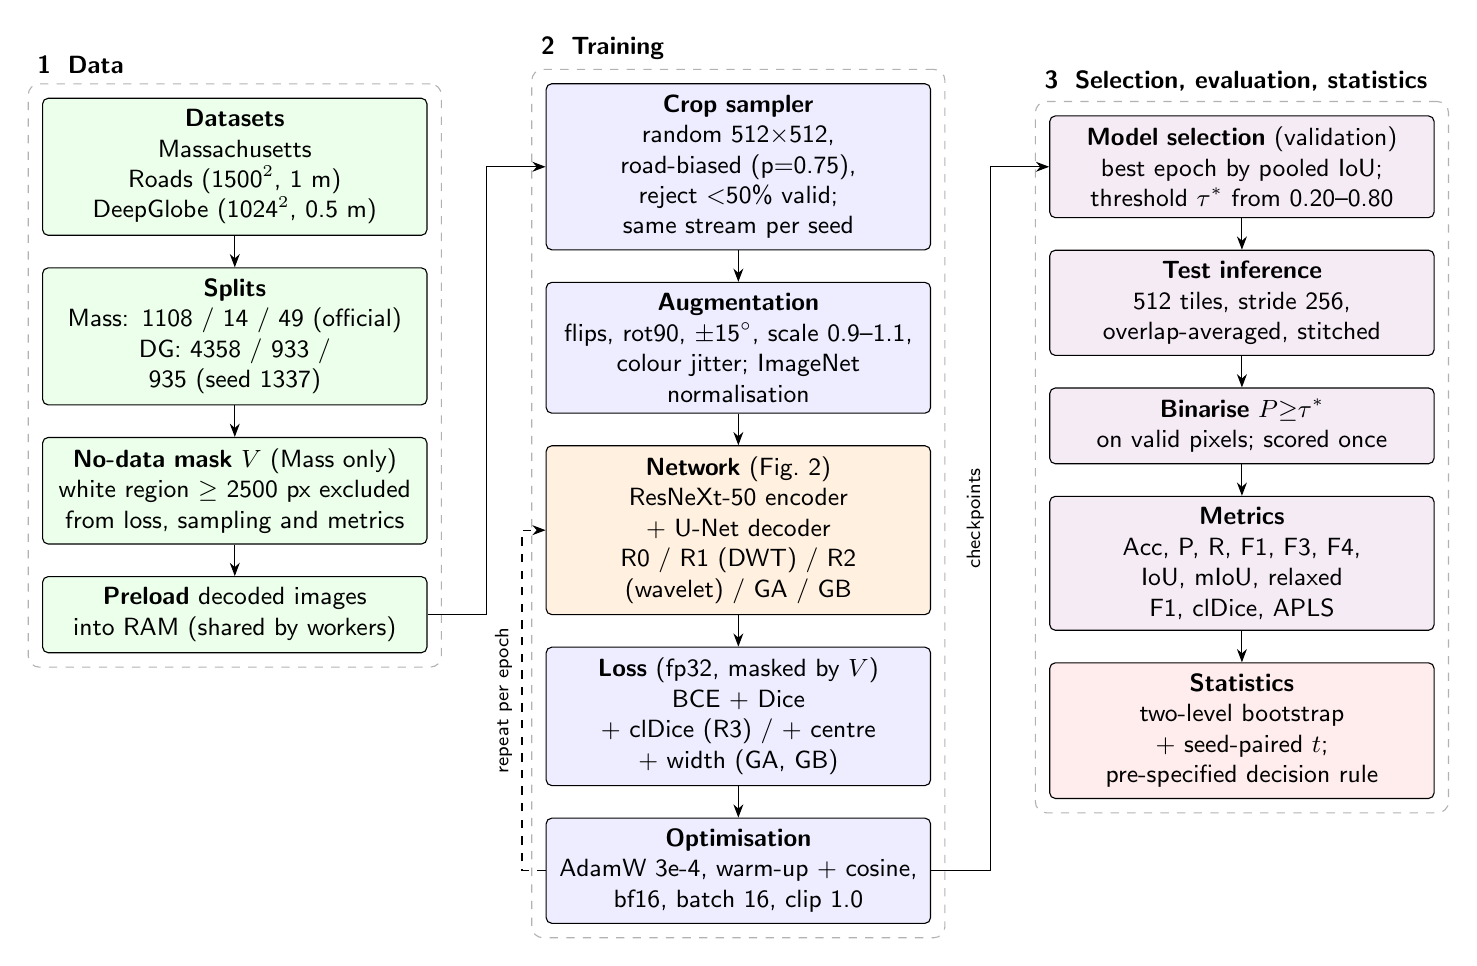
\begin{tikzpicture}[
  font=\sffamily\small, >=Stealth, node distance=4mm and 6mm,
  box/.style={draw, rounded corners=2pt, align=center, inner sep=4pt, text width=#1},
  box/.default=46mm,
  data/.style={box, fill=green!8}, train/.style={box, fill=blue!7},
  model/.style={box, fill=orange!12}, evalb/.style={box, fill=violet!8}, stat/.style={box, fill=red!7},
  lane/.style={draw=gray!60, dashed, rounded corners=4pt, inner sep=5pt},
  lbl/.style={font=\sffamily\bfseries\small, anchor=south west}]

% ---------------- column 1: data
\node[data] (ds) {\textbf{Datasets}\\Massachusetts Roads (1500$^2$, 1 m)\\DeepGlobe (1024$^2$, 0.5 m)};
\node[data, below=of ds] (split) {\textbf{Splits}\\Mass: 1108 / 14 / 49 (official)\\DG: 4358 / 933 / 935 (seed 1337)};
\node[data, below=of split] (nodata) {\textbf{No-data mask} $V$ (Mass only)\\white region $\geq$ 2500 px excluded\\from loss, sampling and metrics};
\node[data, below=of nodata] (preload) {\textbf{Preload} decoded images\\into RAM (shared by workers)};

% ---------------- column 2: training
\node[train, right=15mm of ds] (crop) {\textbf{Crop sampler}\\random 512$\times$512, road-biased (p=0.75),\\reject $<$50\% valid; same stream per seed};
\node[train, below=of crop] (aug) {\textbf{Augmentation}\\flips, rot90, $\pm$15$^\circ$, scale 0.9--1.1,\\colour jitter; ImageNet normalisation};
\node[model, below=of aug] (net) {\textbf{Network} (Fig.~2)\\ResNeXt-50 encoder + U-Net decoder\\R0 / R1 (DWT) / R2 (wavelet) / GA / GB};
\node[train, below=of net] (loss) {\textbf{Loss} (fp32, masked by $V$)\\BCE + Dice\\{}+ clDice (R3) / + centre + width (GA, GB)};
\node[train, below=of loss] (opt) {\textbf{Optimisation}\\AdamW 3e-4, warm-up + cosine,\\bf16, batch 16, clip 1.0};

% ---------------- column 3: selection, inference, evaluation
\node[evalb, right=15mm of crop] (sel) {\textbf{Model selection} (validation)\\best epoch by pooled IoU;\\threshold $\tau^*$ from 0.20--0.80};
\node[evalb, below=of sel] (tile) {\textbf{Test inference}\\512 tiles, stride 256,\\overlap-averaged, stitched};
\node[evalb, below=of tile] (thr) {\textbf{Binarise} $P{\geq}\tau^*$\\on valid pixels; scored once};
\node[evalb, below=of thr] (met) {\textbf{Metrics}\\Acc, P, R, F1, F3, F4,\\IoU, mIoU, relaxed F1, clDice, APLS};
\node[stat, below=of met] (st) {\textbf{Statistics}\\two-level bootstrap + seed-paired $t$;\\pre-specified decision rule};

\draw[->] (ds) -- (split); \draw[->] (split) -- (nodata); \draw[->] (nodata) -- (preload);
\draw[->] (crop) -- (aug); \draw[->] (aug) -- (net); \draw[->] (net) -- (loss); \draw[->] (loss) -- (opt);
\draw[->] (sel) -- (tile); \draw[->] (tile) -- (thr); \draw[->] (thr) -- (met); \draw[->] (met) -- (st);
\draw[->] (preload.east) -- ++(7.5mm,0) |- (crop.west);
\draw[->, dashed] (opt.west) -- ++(-3mm,0) |- (net.west);
\node[font=\sffamily\scriptsize, rotate=90, anchor=south] at ($(opt.west)!0.5!(net.west)+(-3mm,0)$) {repeat per epoch};
\draw[->] (opt.east) -- ++(7.5mm,0) |- (sel.west);
\coordinate (cmid) at ($(opt.east)!0.5!(sel.west)$); \coordinate (cx) at ($(opt.east)+(5.6mm,0)$);
\node[font=\sffamily\scriptsize, rotate=90, anchor=center] at (cx |- cmid) {checkpoints};

\begin{scope}[on background layer]
  \node[lane, fit=(ds)(preload), label={[lbl]north west:1\; Data}] {};
  \node[lane, fit=(crop)(opt), label={[lbl]north west:2\; Training}] {};
  \node[lane, fit=(sel)(st), label={[lbl]north west:3\; Selection, evaluation, statistics}] {};
\end{scope}
\end{tikzpicture}
\end{document}
